\begin{figure}[H]
    \centering
    \begin{subfigure}{0.9\textwidth}
        \centering
        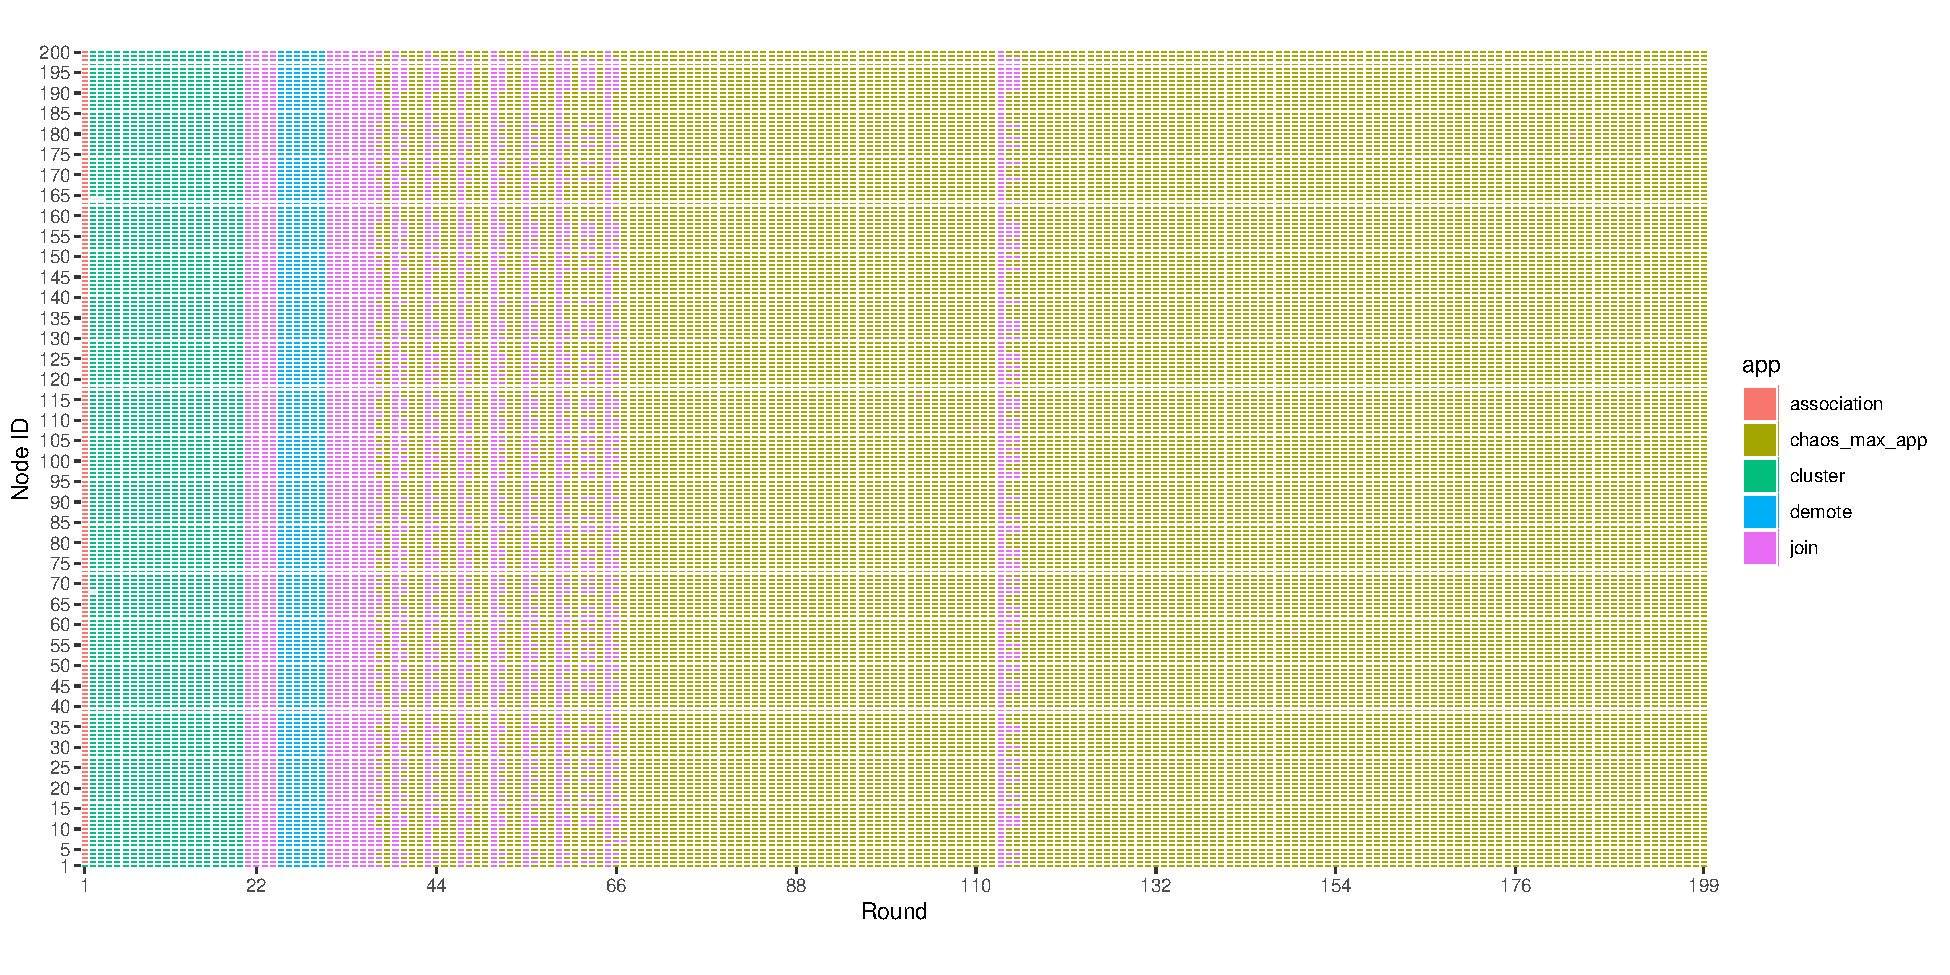
\includegraphics[width=\textwidth]{figure/Results/ReliabilityDiscussionApplicationHeatmaps/applicationmap200x200_1.pdf}
        \label{subfig:application-map-200-nodes-round-1-199}
    \end{subfigure}
    \hfill
    \begin{subfigure}{0.9\textwidth}
        \centering
        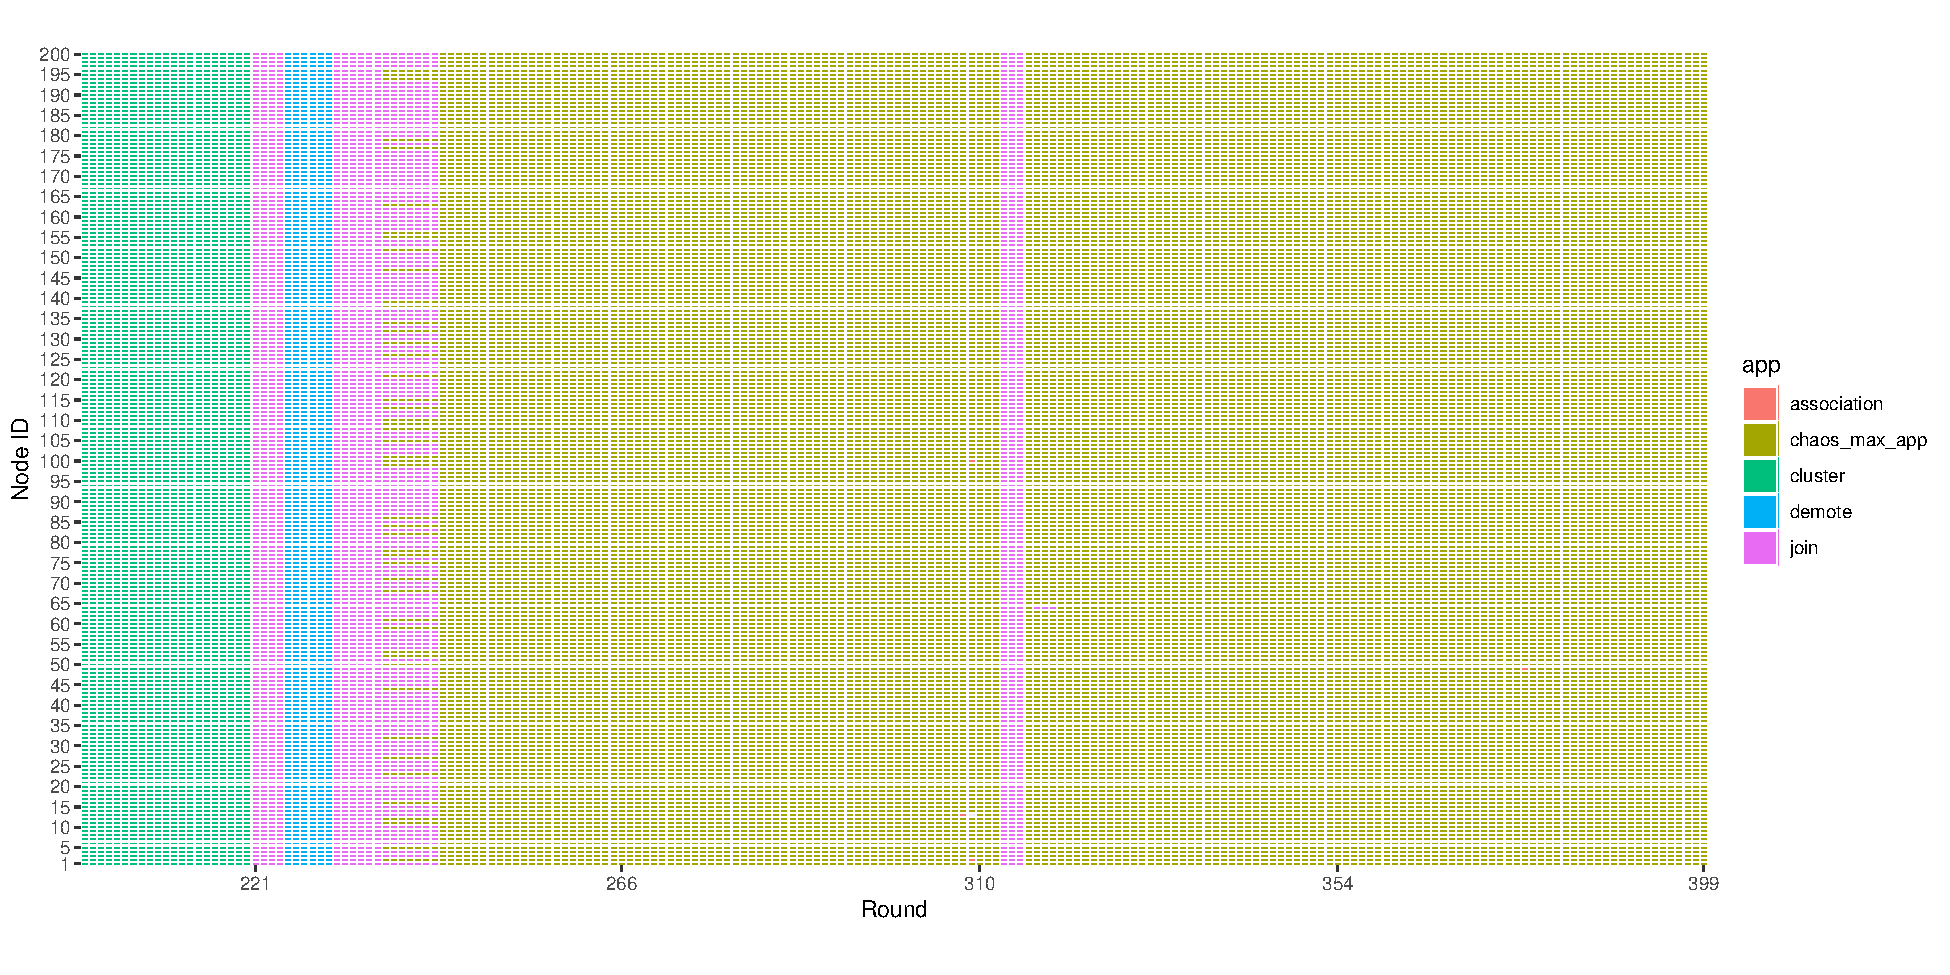
\includegraphics[width=\textwidth]{figure/Results/ReliabilityDiscussionApplicationHeatmaps/applicationmap200x200_2.pdf}
        \label{subfig:application-map-200-nodes-round-200-399}
    \end{subfigure}
    \begin{subfigure}{0.9\textwidth}
        \centering
        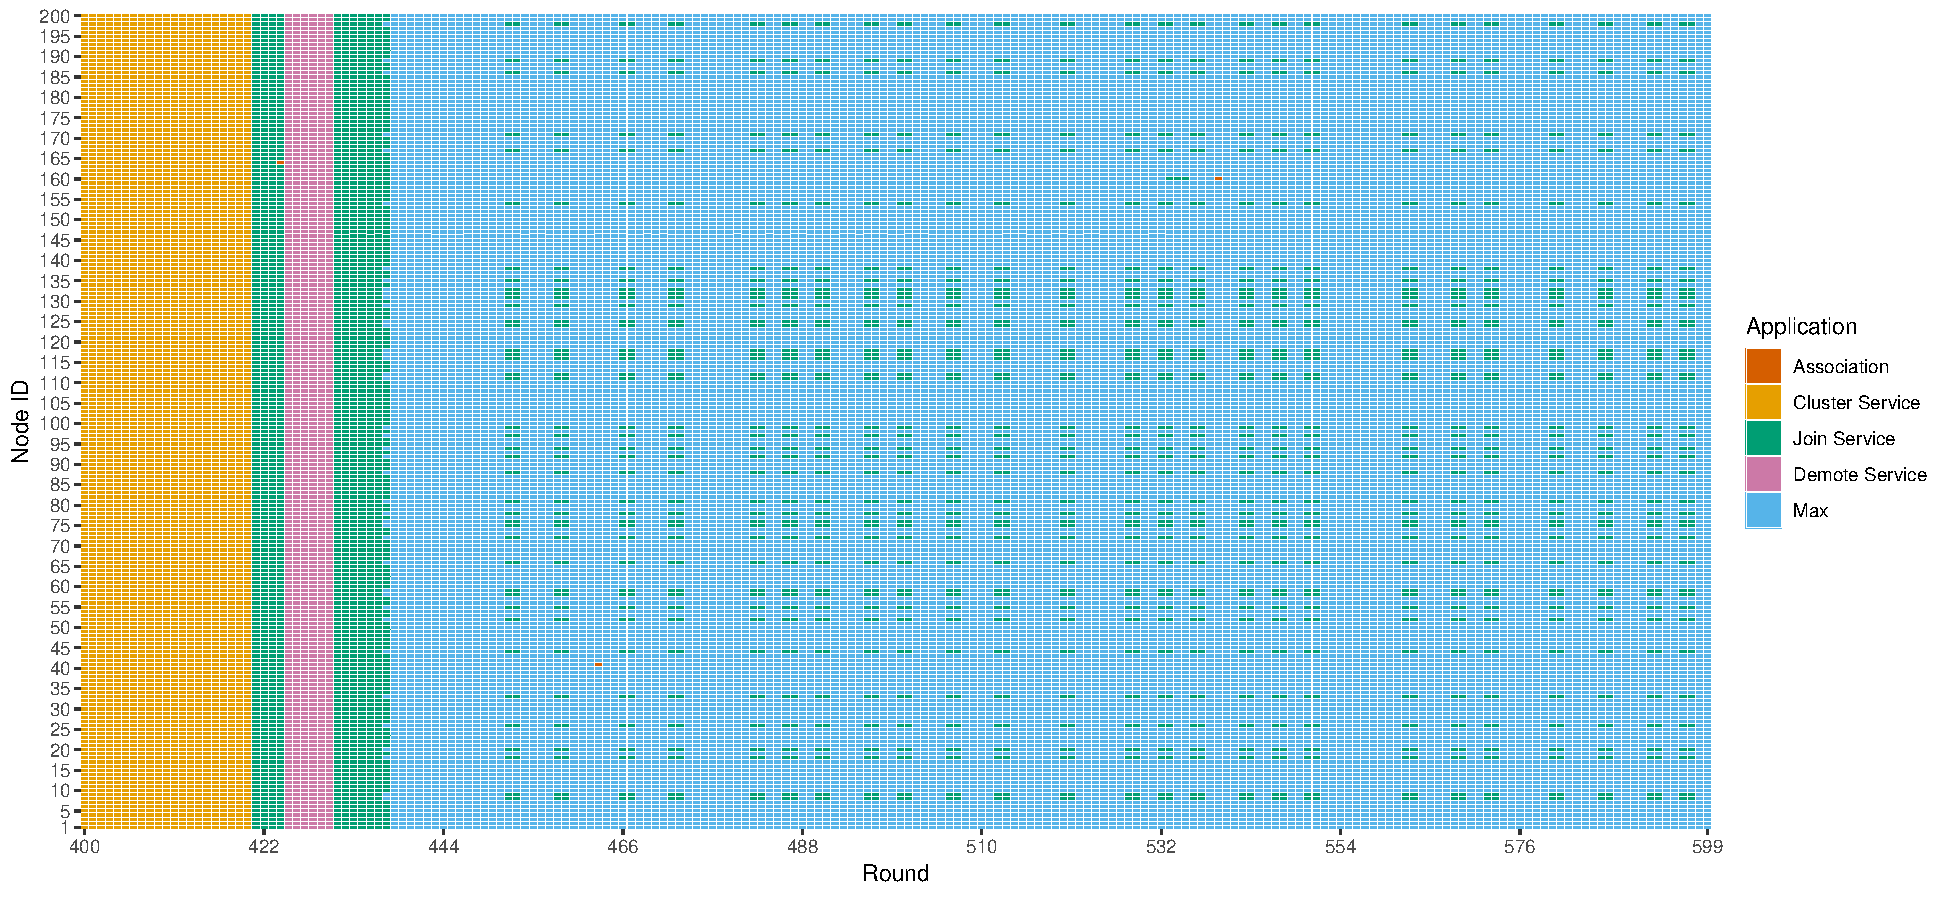
\includegraphics[width=\textwidth]{figure/Results/ReliabilityDiscussionApplicationHeatmaps/applicationmap200x200_3.pdf}
        \label{subfig:application-map-200-nodes-round-400-599}
    \end{subfigure}
    \caption{Application heat map of a test with 200 nodes over a 100x100 network area executing 600 rounds. Some clusters often execute join, especially after the last clustering occurring in rounds 400 to 437}
    \label{fig:application-map-200-nodes}
\end{figure}